\section{Methodology}
\label{sec:methods}

\subsection{Dataset}
\label{subsec:dataset}

The data



\subsection{Preprocessing}
\label{subsec:prepro}
The proposed preprocessing steps for the MRIs consist of: bias correction using the N4ITK algorithm \cite{n4itk}, image normalization to an interval of [0,1], automatic selection of a region of interest (ROI), image re-sampling to a resolution of $0.5 \times 0.5 \times 0.5$ mm, and contour interpolation using optical flow.  

The method for selecting the ROI was originally proposed in \cite{anneke}. It consist of reducing the size of the MRIs (axial, sagittal, and coronal) by cropping the images with the volume that comes from the intersection of the rectangular prisms for the three planes. Resampling is performed using linear interpolation and is programed with the ITK software \cite{itk}.  Figure \ref{fig_1} shows an example of the resulting image after being preprocessed with bias correction, normalization, and cropped to a ROI. 

\begin{figure}[h]
    \centering
    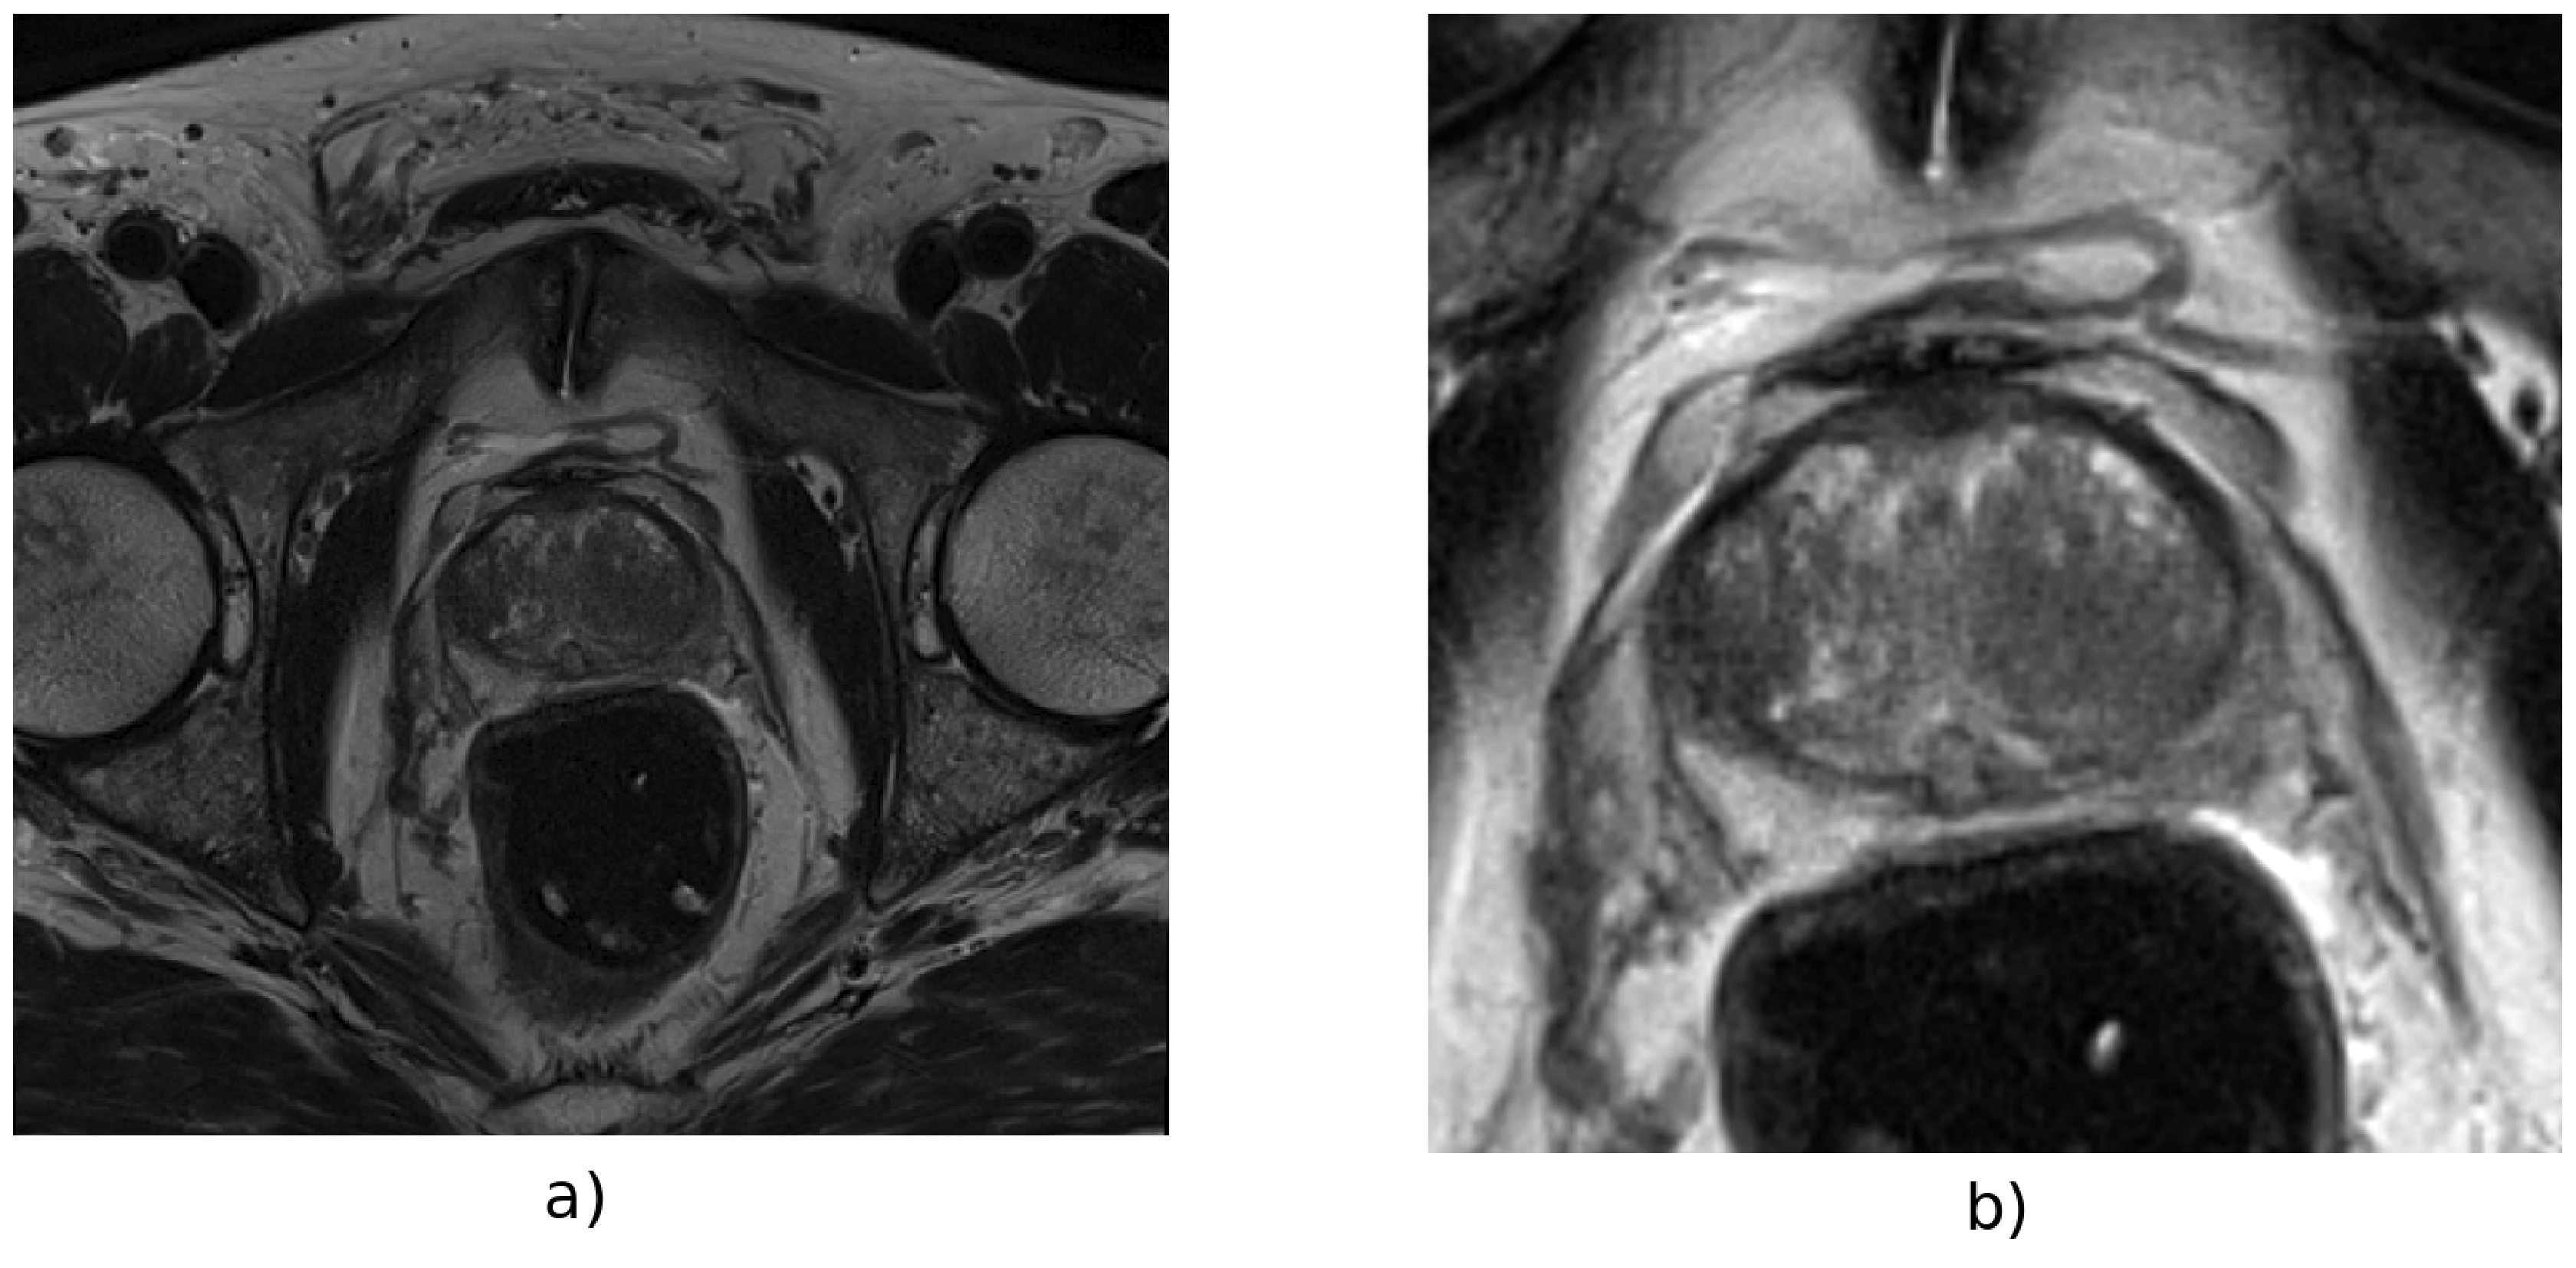
\includegraphics[totalheight=.25\textheight]{figures/Figure1.eps}
    \caption{The MRIs are pre-processed with bias correction, normalization, resampling, and cropped to a ROI to reduce the variability of sizes and intensities between magnets. In this example, \textbf{a)} is the original image and \textbf{b)} is the image after being processed.} 
    \label{fig_1}
\end{figure}

Manual contours made by the experts were carried on the original MRI resolutions and not on the higher resolution version; therefore, the necessity for interpolating them.  The proposed interpolation is performed in two dimensions and is computed independently between every two consecutive horizontal slices. First, optical flow is obtained between the two contours using the Farneback method \cite{optflow}. Then, the contours are interpolated linearly following the direction of the optical flow. Figure \ref{fig:of1} shows an example of the optical flow obtained between two horizontal slices and the resulting interpolated contour using this method. 

\begin{figure}[h]
    \centering
    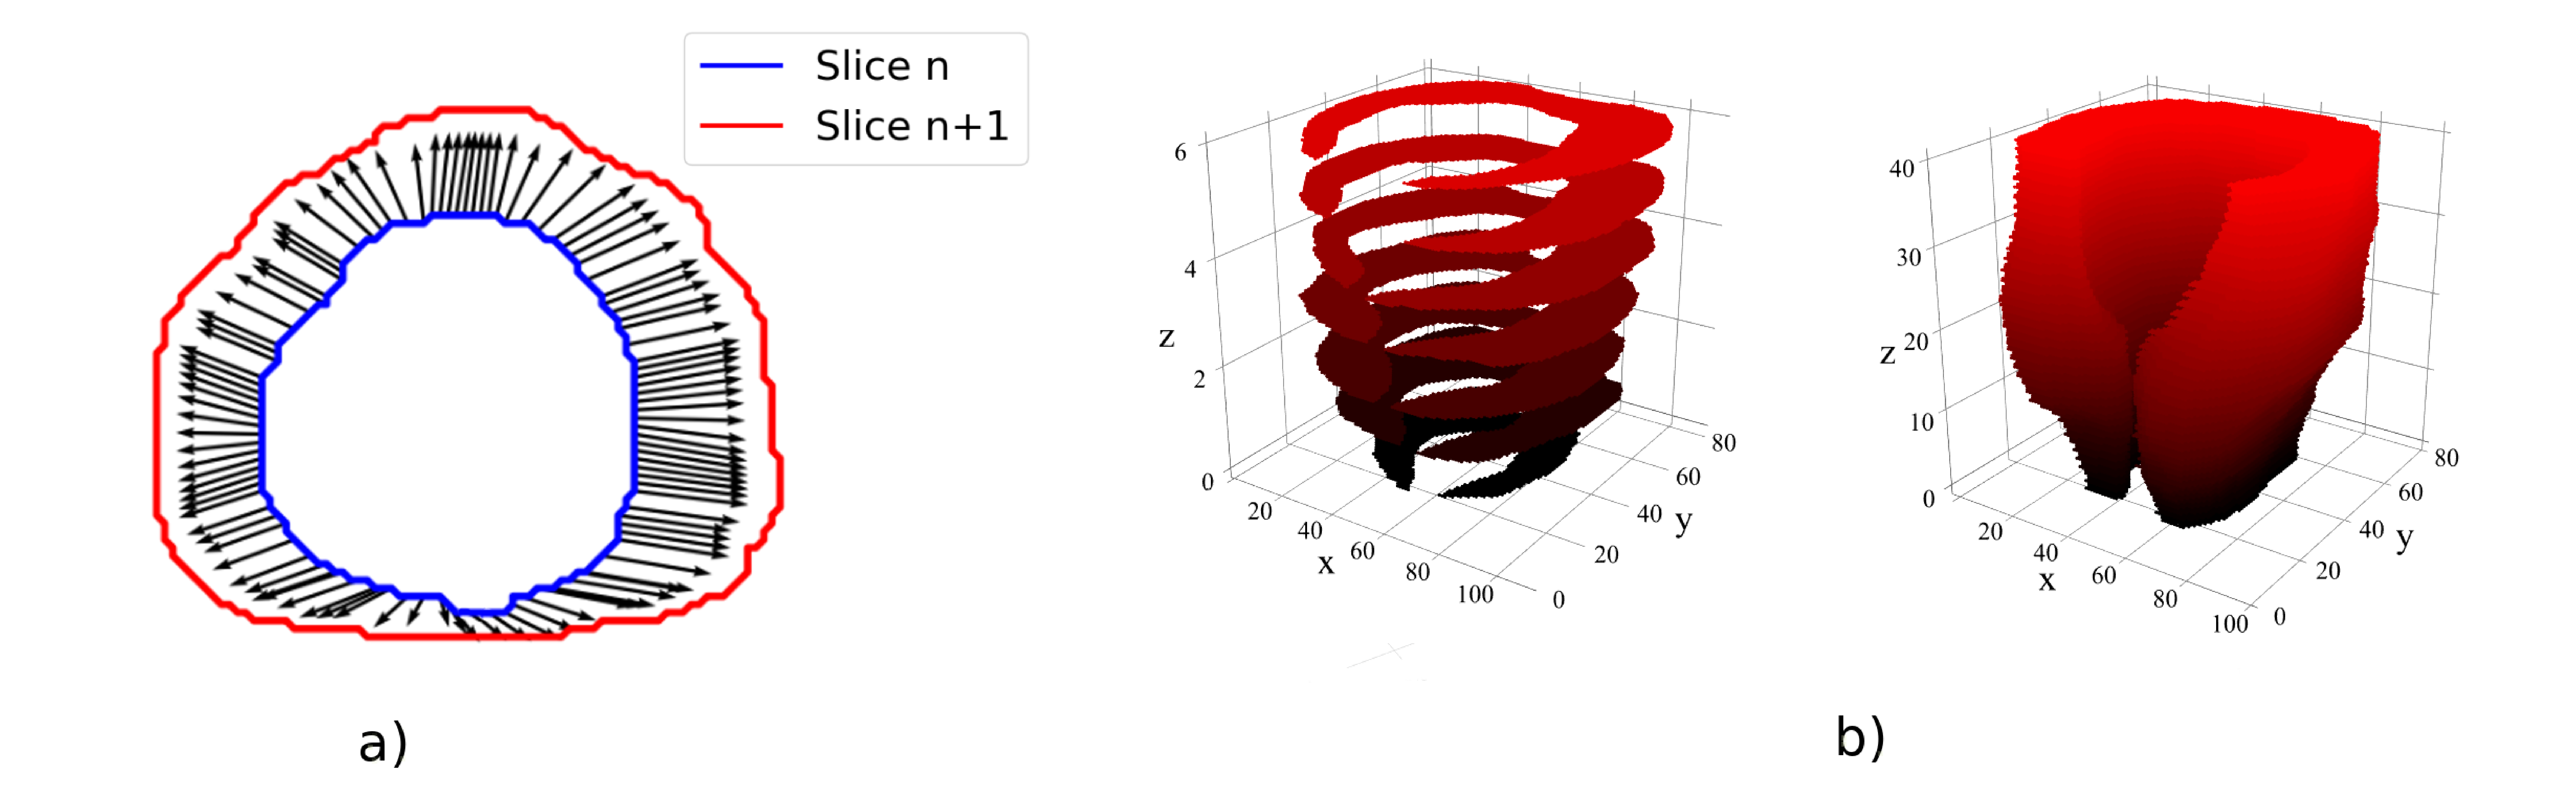
\includegraphics[totalheight=.21\textheight]{figures/Figure2.eps}
    \caption{Example of the proposed algorithm to increase the resolution of prostate and PZ contours. In \textbf{a)}, an example of the optical flow obtained between two prostate contours from adjacent horizontal planes. In \textbf{b)} on the left, original contours with 17 slices. On the right, interpolated contours with 68 slices.}
    %an example of the original resolution contours (made by an expert in the field), and the high resolution contour obtained by interpolating linearly between slices using the vector fields from the optical flow. Contours provided by experts are made on the original resolution of the MRI and interpolated using optical flow and linear interpolation to the higher resolution ROI. }
    \label{fig:of1}
\end{figure}

\subsection{3D-CNN architecture}
The proposed CNN consist of a 3D multistream architecture that follows the analysis and synthesis path of the 3D U-Net \cite{cciccek20163d}. Our implementation follows the one proposed by Anneke et al. in 2018  \cite{anneke}. The input of each stream is the post-processed ROI for one of three MRI scans (axial, sagittal, and coronal), with a resolution of $168^3$. During the analysis phase, a combination of two convolutional layers and one max pool layer is repeated three times. The second convolutional layer in each set doubles the number of channels.  In the synthesis phase, a similar set of two convolutional layers and one deconvolution is applied, followed by batch normalization and Dropout of 20\% \cite{hinton2012improving}. Our contributions
to the original model are: the inclusion of batch normalization layers; the additional Dropout layers, that improves the generalization of the model; and the cut down on the number of filters from $192$ to $28$ in the largest convolutional layer (after the first concatenation) reducing the number of parameters from to 995k to 663k in this layer. Figure \ref{fig:nn} shows the proposed model, all convolutional layers use a filter size of $3 \times 3 \times 3$ and rectified linear unit (ReLu) as the activation function; with the exception of the last layer which uses a filter size of $1 \times 1 \times 1$ and Sigmoid as the activation function. 
\begin{figure*}[h]
    \centering
    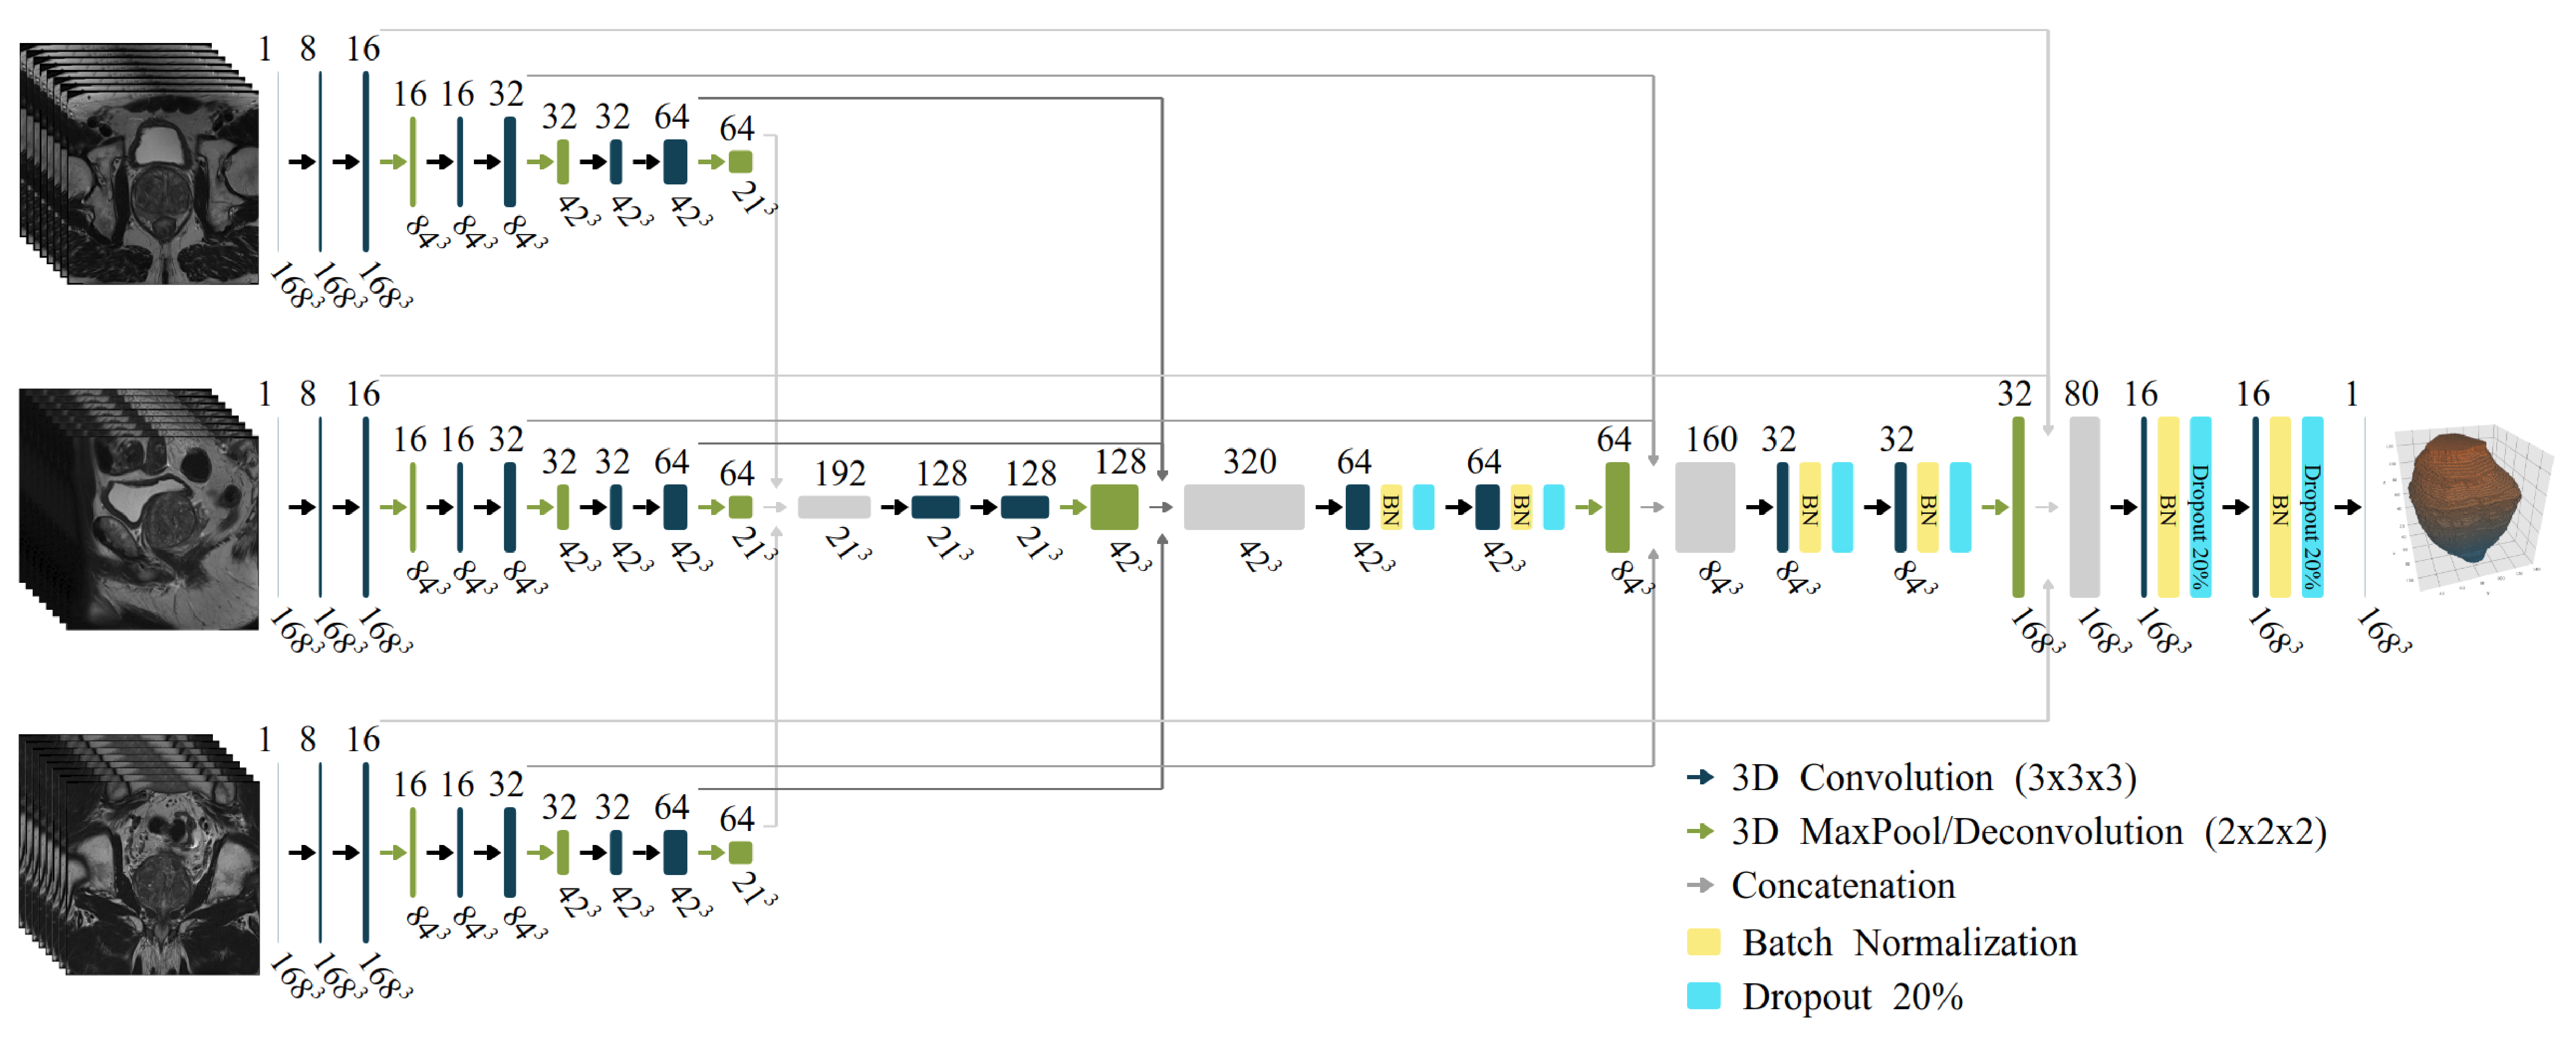
\includegraphics[totalheight=.282\textheight]{figures/Figure3.eps}
    \caption{Multistream 3D convolutional network architecture. The input of the network are three $168^3$ volumes from the MRI planes: axial, sagittal, and coronal. }
    \label{fig:nn}
\end{figure*}

With the proposed architecture the training time is reduced in half, compared to the original architecture of Meyer et al. \cite{anneke}. The improvement is obtained by reducing the total number of parameters, and by adding batch normalization after every convolutional layer in the synthesis path.

\subsection{Training}
\label{subsec:training}
The selected optimization algorithm is Stochastic Gradient Descent (SGD) with a learning rate $\alpha = 0.01$, momentum of 0.9 and decay of $10^{-6}$. The training is performed for 1000 epochs with an early stop mechanism if the loss function is not improved by at least $\delta = 0.001$ after 70 iterations. 

The loss function used for the training is the negative Dice Similarity Coefficient (DSC):
\begin{equation}
\text{Loss} = \frac{2 \sum_{i=1}^{N}p_it_i}{\sum_{i=1}^{N}p_i^2 + \sum_{i=1}^{N}t_i^2 + \varepsilon} 
\label{eq:dsc}
\end{equation}
%where N is the total number of voxels in the image, when training for prostate segmenation,
%and the number of voxels \textbf{inside} the prostate, when training for the PZ. The segmentation
%of the PZ assumes that we already know where the prostate is, so we do not take into
%account anything outside the prostate for the loss function. 
where N is the total number of voxels in the image, $p_i$ the voxel values for the prediction of the network, and $t_i$ the true voxel values of the prostate or PZ masks.

In order to compare the robustness of the models with respect to changes in MRI vendor machines,  a distinct model was trained for each dataset: GE (n=220), Siemens (n=330), combined model (n=550). Each dataset was split into 90\% for training and 10\% for validation. Data augmentation was performed on the fly by flipping the images in the sagittal axis and blurring them using 3D Gaussian blur up to $\sigma = 3$. Each data augmentation method is applied with a random chance of $1/2$.  
A total number of 6 models were trained from the combination of three datasets, and training for the segmentation of the prostate or the PZ. 
